% !TEX root=../main.tex
\chapter{One-Class Neural Networks for Anomaly Detection}
\label{chpt:ocnn}
\section{Introduction}

A common need when analysing real-world datasets is determining which instances stand out as being dissimilar to all others. Such instances are known as \emph{anomalies}, and the goal of \emph{anomaly detection} (also known as \emph{outlier detection}) is to determine all such instances in a data-driven fashion~\cite{chandola2007outlier}. Anomalies can be caused by errors in the data but sometimes are indicative of a new, previously unknown, underlying process; in fact Hawkins~\cite{hawkins1980identification} defines an outlier as an observation that {\it deviates so significantly from other observations as to arouse suspicion that it was generated by a different mechanism.}

Unsupervised anomaly detection techniques uncover anomalies in an unlabeled test data, which plays a pivotal role in a variety of applications, such as, fraud detection, network intrusion detection and fault diagnosis. One-class Support Vector Machines (OC-SVM)~\cite{scholkopf2002support,tax2004support} are widely used, effective unsupervised techniques to identify anomalies. However, performance of OC-SVM is sub-optimal on complex, high dimensional datasets~\cite{vapnik1998statistical,vishwanathan2003simplesvm,bengio2007scaling}.
From recent literature, unsupervised anomaly detection using deep learning is proven to be very effective~\cite{zhou2017anomaly,chalapathy2017robust}. Deep learning methods for anomaly detection can be broadly classified into model architecture using autoencoders~\cite{andrews2016detecting} and hybrid models~\cite{erfani2016high}. Models involving autoencoders utilize magnitude of residual vector (i,e reconstruction error) for making anomaly assessments. While hybrid models mainly use autoencoder as feature extractor, wherein the hidden layer representations are used as input to traditional anomaly detection algorithms such as one-class SVM (OC-SVM). Following the success of transfer learning~\cite{pan2010survey} to obtain rich representative features, hybrid models have adopted pre-trained transfer learning models to obtain features as inputs to anomaly detection methods. Although using generic pre-trained networks for transfer learning representations is efficient, learning representations from scratch, on a moderately sized dataset, for a specific task of anomaly detection is shown to perform better~\cite{andrews2016transfer}. Since the hybrid models extract deep features using an autoencoder and then feed it to a separate anomaly detection method like OC-SVM, they fail to influence representational learning in the hidden layers. In this paper, we build on the theory to integrate a OC-SVM equivalent objective into the neural network architecture. The OC-NN combines the ability of deep networks to extract progressively rich representation of data alongwith the one-class objective, which obtains the hyperplane to separate all the normal data points from the origin. The OC-NN approach is novel for the following crucial reason:  data representation ,is driven by the OC-NN objective and is thus customized for anomaly detection. We show that OC-NN can achieve comparable or better performance in some scenarios than existing shallow state-of-the art methods for complex datasets, while having reasonable training and testing time compared to the existing methods.
%R Hidden layer activations
% in the hidden layer as illustrated in Figure~\ref{fig:h_activations}
% \begin{figure}[t]
%     \centering
%     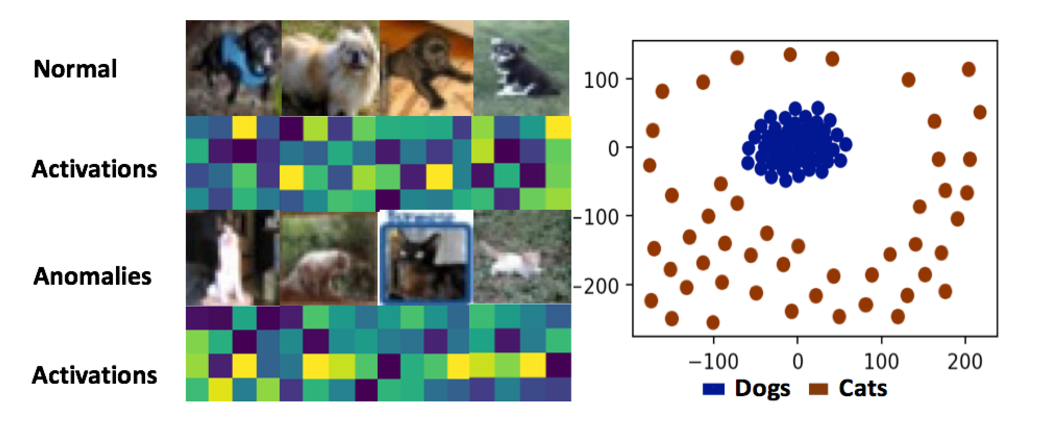
\includegraphics[width=0.8\textwidth]{images/activations}
%     \caption{Hidden layer (sigmoid) activations and its t-sne~\cite{tSNEVisualize2008} embeddings of OC-NN model for CIFAR-10 dataset.}
%     \label{fig:h_activations}
%     \vspace{-0.530cm}
% \end{figure}

We summarize our main contributions as follows:
\begin{itemize}
\item We derive a new one class neural network (OC-NN) model for anomaly detection. OC-NN uses a one class SVM like loss function to drive the training
of the neural network.
\item We propose an alternating minimization algorithm for learning the parameters of the OC-NN model. We observe that the subproblem of
the OC-NN objective is equivalent to a solving a quantile selection problem.
\item We carry out extensive experiments which convincingly demonstrate  that OC-NN  outperforms other state-of-the-art deep learning approaches
for anomaly detection on complex image and sequence data sets.
\end{itemize}

The rest of the paper is structured as follows. In Section~\ref{sec:background} we provide a detailed survey of related and relevant
work on anomaly detection. The main OC-NN model is developed in Section~\ref{sec:method}. The experiment setup, evaluation metrics and
model configurations are described in Section~\ref{sec:experiment-setup}. The results and analysis of the experiments are the focus of
Section~\ref{sec:experiment-results}. We conclude in Section~\ref{sec:conclusion} with a summary and directions for future work.

